\documentclass[11pt,letterpaper]{article}
\usepackage[margin=.72in,top=.70in,bottom=.65in,headsep=17pt]{geometry}
\usepackage[T1]{fontenc}
\usepackage{lmodern,microtype,graphicx,xcolor,amsmath,amssymb,booktabs,tabularx,enumitem,tcolorbox,fancyhdr,ragged2e}
\usepackage[linkcolor=teal,urlcolor=teal,colorlinks=true]{hyperref}
\definecolor{ink}{HTML}{192B36}
\definecolor{muted}{HTML}{526474}
\definecolor{teal}{HTML}{13727C}
\definecolor{aqua}{HTML}{E9F3F3}
\definecolor{bluegrey}{HTML}{F1F5F7}
\definecolor{copper}{HTML}{B46C45}
\definecolor{line}{HTML}{CAD7DB}
\setlength{\parindent}{0pt}
\setlength{\parskip}{.42em}
\setlist[itemize]{leftmargin=1.2em,topsep=2pt,itemsep=2pt,parsep=0pt}
\setlength{\headheight}{13.5pt}
\pagestyle{fancy}\fancyhf{}
\fancyhead[L]{\color{muted}\scriptsize\textsc{Exact Addressing / Scientific Hypothesis Generation}}
\fancyhead[R]{\color{muted}\scriptsize\textsc{Three Stories / Corrected Pilot}}
\fancyfoot[L]{\color{muted}\scriptsize A fictional, retrospectively documented experiment --- not medical advice}
\fancyfoot[R]{\color{muted}\scriptsize\thepage}
\renewcommand{\headrulewidth}{.3pt}
\tcbset{boxrule=0pt,colback=aqua,colframe=aqua,arc=1mm,boxsep=4pt,left=9pt,right=9pt,top=7pt,bottom=7pt}
\newcommand{\eyebrow}[1]{{\textcolor{teal}{\scriptsize\bfseries\MakeUppercase{#1}}}\par\vspace{3pt}}
\newcommand{\hsec}[1]{\vspace{4pt}{\large\bfseries\color{ink}#1}\par\vspace{2pt}{\textcolor{teal}{\rule{.44in}{1.25pt}}}\par\vspace{2pt}}
\newcommand{\numtag}[1]{\textcolor{teal}{\bfseries\small #1}\quad}
\newcommand{\thin}{{\color{line}\rule{\linewidth}{.4pt}}}
\newcommand{\src}[1]{\textsuperscript{\textcolor{teal}{[#1]}}}
\hypersetup{pdftitle={From Leg Pain to Eureka: The Actual Search in the House Three Stories Pilot},pdfauthor={Research companion for Exact Addressing},pdfsubject={Corrected account of incremental diagnostic hypothesis search using Sol and DATA MIND discovery control, citations and image attribution}}
\begin{document}
\vspace*{4pt}
\eyebrow{House, M.D. / ``Three Stories'' / Exact Addressing companion}
{\fontsize{28}{31}\selectfont\bfseries\color{ink}From ``Leg Pain'' to Eureka}\par\vspace{4pt}
{\fontsize{13}{17}\selectfont\color{muted}What Sol and DATA MIND discovered \emph{before} the answer was revealed}\par\vspace{9pt}
\thin\vspace{6pt}

\noindent\begin{minipage}[t]{.47\linewidth}
\vspace{0pt}
\eyebrow{The original starting point}
\begin{tcolorbox}[colback=ink,colframe=ink]
\centering\textcolor{white}{\fontsize{25}{30}\selectfont\bfseries Leg pain.}\par\vspace{3pt}
{\small\color{white}Two words---not a disclosed disease, causal explanation, or known answer.}
\end{tcolorbox}
\small
In the first reported test of \emph{Sol} under \emph{DATA MIND discovery control}, the researcher supplied a fictional patient's evidence \textbf{in stages}. The researcher knew the outcome of the \emph{House, M.D.} episode ``Three Stories''; Sol, according to the participant's retrospective account, was \emph{not} given the reference diagnosis or told the episode's identity during the live diagnostic exchange.\src{1}

\textbf{The experiment was not a jump from an almost-complete diagnosis to the final answer.} Ordinary hypotheses were generated, challenged by additional evidence, and judged to have stalled. Only \emph{then} did one deliberately restricted Eureka prompt produce a different mechanism.\src{1}

\textbf{Terminology:} ``Leg pain'' is the \emph{starting problem statement} (or seed hypothesis, in the researcher's informal usage), not a specific medical diagnosis. The later Eureka \emph{mechanistic hypothesis} and the still-later \emph{episode reveal} occupy different stages.

\vspace{5pt}
\eyebrow{Episode identification}
{\small \emph{House, M.D.}, Season 1, Episode 21, ``Three Stories''; written by David Shore, directed by Paris Barclay; first broadcast on Fox, May 17, 2005.\src{2,3}}
\end{minipage}\hfill
\begin{minipage}[t]{.495\linewidth}
\vspace{0pt}
\IfFileExists{house_character_illustration.jpg}{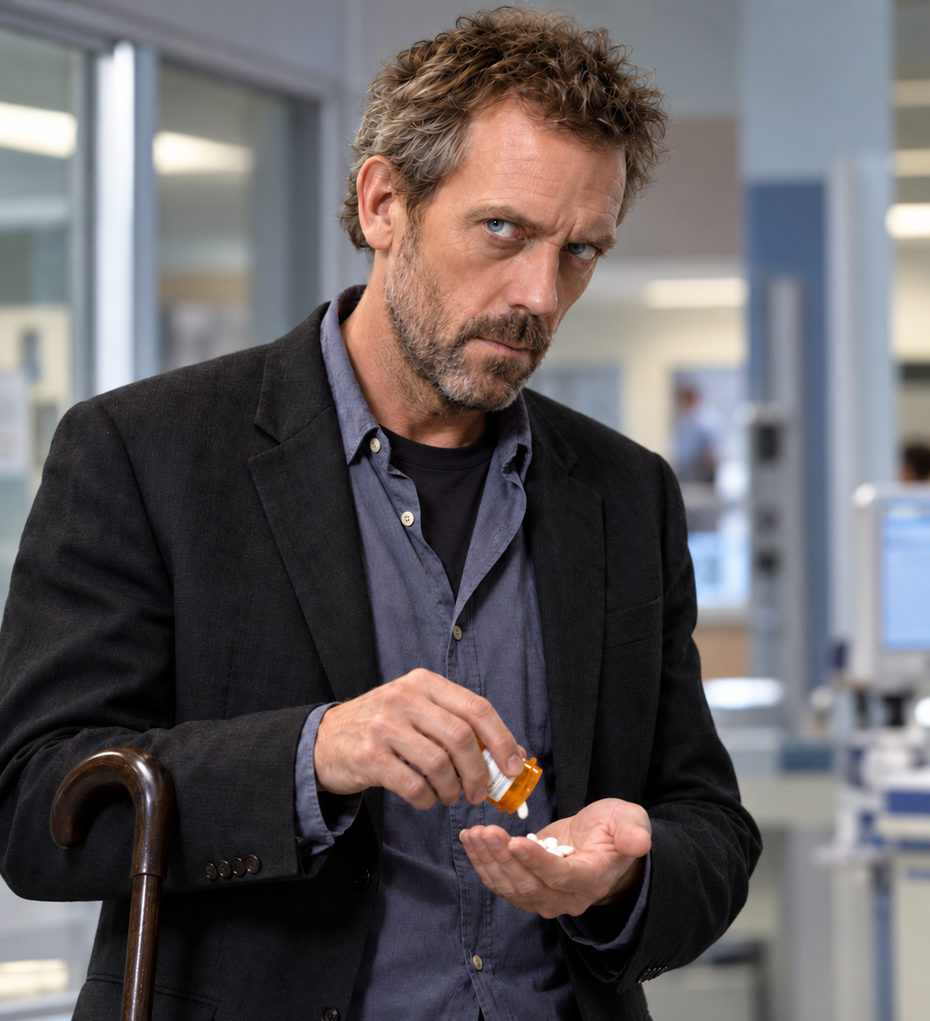
\includegraphics[width=\linewidth,height=5.08in,keepaspectratio]{house_character_illustration.jpg}}{\fcolorbox{line}{bluegrey}{\parbox[c][4.92in][c]{.91\linewidth}{\centering\large\bfseries House, M.D.\\[9pt]\normalsize\mdseries Illustration omitted from this public build; illustrator and reuse license unverified.}}}\par\vspace{5pt}
{\fontsize{8.1}{10}\selectfont\color{muted}\textbf{Figure 1.} Supplied editorial illustration depicting Dr. Gregory House, not an authenticated frame from ``Three Stories.'' Original file: \emph{Dr. House Dispensing Medication in Hospital.png}. Character/series rights credited in the supplied caption to \emph{House, M.D.}/Universal Television; the illustration's artist and license are not identified.\src{4}}
\end{minipage}

\vspace{9pt}
\begin{tcolorbox}[colback=bluegrey]
\small\textbf{The paper's relevant question:} When a conventional candidate search stops making explanatory progress, can a \emph{single evidence-conditioned mechanism-changing hypothesis} escape the basin before a held-back reference explanation is disclosed? The case illustrates that question; it does not constitute a blinded clinical trial or a measured search-speedup theorem.\src{1,5}
\end{tcolorbox}

\newpage
\eyebrow{The experiment reconstructed / before the reveal}
{\fontsize{23}{27}\selectfont\bfseries\color{ink}The search mattered}\par\vspace{4pt}
{\color{muted}The steps between ``leg pain'' and the Eureka result are the result's context---not expendable background.}\par\vspace{7pt}
\hsec{The evidence was released incrementally}
\noindent\begin{minipage}[t]{.485\linewidth}\small
\numtag{00} \textbf{Seed:} ``Leg pain.'' No pathological mechanism is supplied.

\numtag{01} \textbf{Onset:} Sudden, unilateral pain, later described as extremely severe (approximately 9--10/10).

\numtag{02} \textbf{Anatomy:} Focal, mid-thigh location with no radiation.

\numtag{03} \textbf{Appearance and perfusion:} Leg looks essentially normal; distal pulses are preserved.

\numtag{04} \textbf{History:} No injury, trauma, exercise, or triggering movement.
\end{minipage}\hfill\begin{minipage}[t]{.485\linewidth}\small
\numtag{05} \textbf{Function:} Inability to bear weight and diffuse tenderness.

\numtag{06} \textbf{Provocation:} Both muscle contraction and stretching increase pain.

\numtag{07} \textbf{Negative clues:} No swelling, firm or tense thigh, or anticoagulant use.

\numtag{08} \textbf{Residual puzzle:} Severe focal thigh pain remains disproportionately unexplained by the ordinary candidate families.

{\color{muted}\footnotesize Sequence condensed from the supplied narrative; it is not a recovered timestamped prompt transcript.\src{1}}
\end{minipage}

\vspace{8pt}
\hsec{Ordinary differential search did real work}
\small
The search first considered familiar explanatory families: \textbf{acute arterial ischemia, compartment syndrome, deep-vein thrombosis (DVT), musculoskeletal injury, neurologic/radicular pain, and infection}. Subsequent information weakened some familiar presentations: normal appearance and preserved distal pulses made a major occlusion less obvious; no trauma or exertion weakened ordinary strain; focal nonradiating pain weakened radicular explanations; no swelling or tenseness weakened classic compartment syndrome.\src{1}

\begin{tcolorbox}[colback=bluegrey]
\small\textbf{Important qualification.} These were \emph{changes in plausibility}, not formal exclusions. For example, preserved distal pulses do not logically rule out localized muscle ischemia. The description is a report of a fictional search, not medical triage guidance.
\end{tcolorbox}

\hsec{Then the candidate search entered a basin}
\small
The model had not enumerated all diseases. Rather, the ordinary differential was generating variants of already-considered mechanisms \emph{without explaining their shared residual}: abrupt onset, extreme focal thigh pain, little visible abnormality, preserved pulses, and no precipitating injury. The participant recognized this as a \textbf{search basin} and chose to change the search policy. The Eureka intervention occurred \emph{before} the episode's full answer was disclosed.\src{1}

\begin{tcolorbox}
\centering\small\bfseries\color{ink}EVIDENCE $\longrightarrow$ ORDINARY SEARCH $\longrightarrow$ RESIDUAL PATTERN $\longrightarrow$ BASIN
\end{tcolorbox}

\newpage
\eyebrow{Eureka intervention / withheld-answer comparison}
{\fontsize{23}{27}\selectfont\bfseries\color{ink}One hypothesis, then the reveal}\par\vspace{6pt}
\hsec{The one-candidate depth charge}
\small
The researcher's instruction was \emph{approximately}: ``Generate exactly one new mechanistic hypothesis outside the ordinary explanations. Explain what tissue or process could cause the presentation, and give one finding or test that would discriminate it.'' The wording is a retrospective approximation, not a verified verbatim exchange. Its operative constraint was \textbf{one new mechanism, not ten more guesses}.\src{1}

\begin{tcolorbox}[colback=aqua]
\eyebrow{Sol's Eureka hypothesis / before the hidden answer}
{\fontsize{17}{20}\selectfont\bfseries\color{ink}Spontaneous skeletal-muscle infarction / myonecrosis}\par\vspace{4pt}
\small Severe localized ischemic muscle injury could cause striking pain with contraction or stretching even while the leg looked relatively normal and distal pulses remained present. Sol proposed muscle-focused imaging, particularly MRI, as a possible discriminator.\src{1}
\end{tcolorbox}
\small
The account records the researcher saying \textbf{``SAY EUREKA''}, followed by \textbf{``THAT'S CORRECT.''} The confirmed correspondence was with the \emph{pathological class}---not yet the full upstream vascular cause.\src{1}

\hsec{Only afterward: the television episode's fuller diagnosis}
\small
In ``Three Stories,'' one apparently drug-seeking patient's pain is ultimately revealed as House's own history. The plot explanation is a clot-associated aneurysm that obstructed circulation, caused thigh-muscle infarction, and led to tissue necrosis and lasting injury. Later details include dark urine, attempts at treatment, muscle removal and chronic pain.\src{2,3}

\begin{tcolorbox}[colback=bluegrey]
\centering\small\textbf{EPISODE REVEAL (NOT THE INITIAL INPUT)}\par\vspace{6pt}
{\normalsize\bfseries\color{ink}aneurysm $\to$ thrombus $\to$ arterial obstruction}\par\vspace{2pt}
{\normalsize\bfseries\color{ink}ischemia $\to$ muscle infarction $\to$ necrosis}\par\vspace{5pt}
{\scriptsize\color{muted}The Eureka proposal anticipated the tissue-level mechanism, but not the entire causal origin.}
\end{tcolorbox}
\vspace{2pt}
\hsec{Two hypotheses at two different depths}
\small
\textbf{$H_1$ (Eureka output):} localized skeletal-muscle infarction / ischemic myonecrosis.

\textbf{$H_2$ (later, fuller explanation):} a thrombosed aneurysm producing arterial obstruction and muscle infarction.

In this narrative, $H_2$ \emph{contains and explains} the pathological process $H_1$, while $H_1$ alone does not identify $H_2$. Thus \textbf{fit to the evidence does not imply explanatory completeness}. This directional explanatory relationship is not the claim that $H_1$ logically forces an aneurysm.\src{1,5}

\newpage
\eyebrow{Research interpretation / references}
{\fontsize{23}{27}\selectfont\bfseries\color{ink}Why the result was interesting}\par\vspace{5pt}
\hsec{The method, not a lucky late guess}
\small
The contribution is the \emph{sequence and timing}: evidence accumulation first; ordinary search that genuinely constrains the problem; a recognized stagnation basin; exactly one evidence-conditioned mechanism-changing candidate; a proposed discriminator; and only then a comparison with the concealed fictional reference explanation. A jump from ``muscle infarction'' to ``thrombosed aneurysm'' would miss the actual search experiment.\src{1}

\begin{tcolorbox}[colback=aqua]
\centering
{\small\bfseries\color{ink}LEG PAIN}\par\vspace{1pt}
$\downarrow$\par
{\small staged evidence $\to$ ordinary differential $\to$ search basin}\par\vspace{2pt}
$\downarrow$\par
{\small\bfseries exactly one Eureka / depth-charge hypothesis}\par\vspace{2pt}
$\downarrow$\par
{\small muscle infarction / myonecrosis + proposed discriminator}\par\vspace{2pt}
$\downarrow$\par
{\small later episode reveal + externally compared explanatory depth}
\end{tcolorbox}
\vspace{3pt}
\small
The practical principle suggested by the narrative is \textbf{``Do not depth-charge too early.''} Search diversity is useful \emph{after} conventional candidates have been tested against evidence, not merely because an exotic alternative can be named. A stronger scientific test would freeze the prompts, intermediate evidence and time order; preserve full logs; use independent adjudication; and compare against a predeclared ordinary-search baseline.\src{1,5}

\textbf{Evidence boundary.} This is a retrospective description of a staged fictional exercise. The supplied document is not a raw, immutable interaction log, the clue presenter knew the reference answer, and the proposed MRI was not performed. It demonstrates a \emph{plausible method of directing search}, not verified clinical competence, independent blinding, or a quantified advantage.\src{1}

\hsec{Episode, experiment and figure citations}
{\fontsize{8.5}{11.0}\selectfont\color{muted}
\textbf{[1] Primary account of the experiment.} Brian Tenneson, \emph{First Try Hypothesis Generator: A Differential Diagnosis from House}, participant's retrospective working document supplied October 13, 2026, pp. 1--8. It explicitly identifies the opening words ``Leg pain,'' the progressive evidence, the stalled ordinary differential, the approximate one-candidate instruction, and the later reveal. Not a timestamped verbatim prompt log.

\textbf{[2] Episode (primary audiovisual work).} David Shore (writer) and Paris Barclay (director), ``Three Stories,'' \emph{House, M.D.}, Season 1, Episode 21, Fox, aired May 17, 2005. \href{https://www.paleycenter.org/collection/item/?item=T%3A86070}{Paley Center archive, catalog T:86070}.

\textbf{[3] Episode guide (plot and credits).} \emph{House, M.D. Episode Guide}, ``Season One \#121: Three Stories,'' \href{https://www.housemd-guide.com/season1/121stories.php}{episode synopsis and credits}. See also \href{https://www.imdb.com/title/tt0606046/}{IMDb title tt0606046}.

\textbf{[4] Image provenance and rights notice.} \emph{Dr. House Dispensing Medication in Hospital.png}, editorial depiction from the researcher's supplied Library; image caption credits ``\emph{House, M.D.} (television series), Universal Television.'' Reproduced here as a character illustration, \emph{not} authenticated as a still from this episode. The illustrator, original publication, and reuse license are unverified; character/series attribution is not permission to reproduce the image.

\textbf{[5] Mathematical manuscript.} Brian Tenneson, \emph{Exact Addressing, Proof Geometry, Locality, Verifier-Safe Hilbert Search, and Formalized Scientific Hypothesis Generation}, Preliminary Release 3.3.2, \S14.5 (fictional differential-diagnosis pilot and the evidence-fit/explanatory-completeness distinction), October 13, 2026.
}
\vfill
\thin\par\vspace{3pt}
{\fontsize{8.8}{11}\selectfont\color{muted}Editorial correction: this companion separates the two-word initial problem, the intermediate Eureka mechanism and the later television answer. The unchanged underlying article was not modified by this PDF revision.}
\end{document}